% Unofficial University of Texas at Arlington Math Poster template:

% A fork of the unofficial University of Lethbridge Poster template: https://www.overleaf.com/latex/templates/university-of-lethbridge-unofficial-poster-template/nddfzgvqvfwf
% which is a fork of unofficial University of Alberta Poster template: 
% which is a fork of Yale template: https://www.overleaf.com/latex/templates/yale-poster-template/rjpgqfgvsjcv
% which is a fork of the UMich template https://www.overleaf.com/latex/templates/university-of-michigan-umich-poster-template/xpnqzzxwbjzc
% which is fork of the MSU template https://www.overleaf.com/latex/templates/an-unofficial-poster-template-for-michigan-state-university/wnymbgpxnnwd
% which is a fork of https://www.overleaf.com/latex/templates/an-unofficial-poster-template-for-new-york-university/krgqtqmzdqhg
% which is a fork of https://github.com/anishathalye/gemini
% also refer to https://github.com/k4rtik/uchicago-poster


\documentclass[final]{beamer}

% ====================
% Packages
% ====================

\usepackage[T1]{fontenc}
\usepackage[utf8]{luainputenc}
\usepackage{lmodern}
%\usepackage[size=custom, width=122,height=91, scale=1.2]{beamerposter}
\usepackage[orientation=portrait, size=a0, scale=1.25]{beamerposter}
\usetheme{gemini}
\usecolortheme{msu}
\usepackage{graphicx}
\usepackage{booktabs}
\usepackage{tikz}
\usepackage{pgfplots}
\pgfplotsset{compat=1.14}
\usepackage{anyfontsize}
\usepackage{multirow}
\usepackage{listings}
\usepackage[dvipsnames]{xcolor}
% ====================
% Lengths
% ====================

% If you have N columns, choose \sepwidth and \colwidth such that
% (N+1)*\sepwidth + N*\colwidth = \paperwidth
\newlength{\sepwidth}
\newlength{\colwidth}
\setlength{\sepwidth}{0.025\paperwidth}
\setlength{\colwidth}{0.3\paperwidth}

\newcommand{\separatorcolumn}{\begin{column}{\sepwidth}\end{column}}

% ====================
% Title
% ====================

\title{Implementing FAIR Data Exchange in ACTRIS Switzerland : An Expert-Driven Approach}
%\setbeamerfont{title}{size=\huge}

\author{Juan F. Fl\'orez-Ospina,  Leïla H. Simon, Nora K. Nowak, Benjamin T. Brem, \\ Martin Gysel-Beer, and Robin L. Modini}

%\author{Juan F. Florez-Ospina$^{1}$, Natasha M. Garner$^{1}$, Lucia Iezzi$^{1}$, David Bell$^{1}$,\\ Imad El Haddad$^{1}$, Julia Schmale$^{2}$, and Thorsten Bartels-Rausch$^{1}$}
% add following line if you have co-author(s)
% Coauthor One$^{2}$, Coauthor Two$^{3}$

\institute[shortinst]{PSI Center for Energy and Environmental Sciences, 5232 Villigen PSI, Switzerland}

% ====================
% Footer (optional)
% ====================
\footercontent{\hfill
  \href{mailto:juan.florez-ospina@psi.ch}{juan.florez-ospina@psi.ch, juanflo16@gmail.com,} \href{robin.modini@psi.ch}{robin.modini@psi.ch}}
% (can be left out to remove footer)
%\footercontent{22-Nov-2023, Swiss Data Science Conference, Bern \hfill
%  \href{mailto:juan.florez-ospina@psi.ch}{juan.florez-ospina@psi.ch} \href{thorsten.bartels-rausch@psi.ch}{thorsten.bartels-rausch@psi.ch}}
% (can be left out to remove footer)

% ====================
% Logo
%\logoleft{\includegraphics[height=5.5cm]{logos/psi_01_sn.png}}
% ====================

% use this to include logos on the left and/or right side of the header:
% Left: institution
% \logoright{\includegraphics[height=5cm]{logos/logo-wordmark-variations.png}}
% Right: funding agencies and other affilations 
%\logoright{\includegraphics[height=7cm]{logos/NSF.eps}}

% ====================
% Body
% ====================


\begin{document}

\begin{frame}[t]

\begin{columns}[t]
\separatorcolumn


\begin{column}{1.5\colwidth}

\begin{block}{Motivation}

%Given an \textit{allocated time frame},

\textbf{Problem.} Scientific datasets in atmospheric science are often large, complex and highly specialized, making them hard to reuse across users, tools, and time. 
\textcolor{white}{insert line here :)}

Adhering to the FAIR data principles promises to resolve long term reuse of data by machines and humans.
\textcolor{white}{insert line here :)}

\textbf{Yet in practice,} implementations often have the following configuration,
\vspace{1em} % Add some space before next block

\begin{figure}
\centering
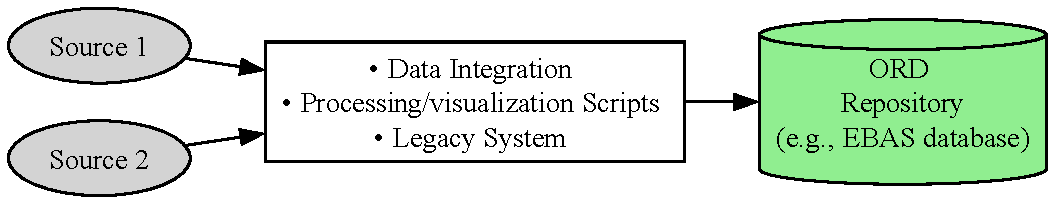
\includegraphics[width=0.75\textwidth]{figures/styled_typical_exchange.pdf}
\caption{Diagram of tightly coupled system for integration, processing and ingestion of scientific data into ORD repositories.}
\end{figure}
which in turn exhibits the following
\vspace{1em}
\begin{exampleblock}{System drawbacks:}
\begin{itemize}
    \item 
    Task-specific outputs, limiting adaptability to new needs or use cases.
    \item 
    Monolithic design, making the system hard to maintain, reuse or understand internally.
    \item 
    Embedded domain knowledge in hard-coded parameters, reducing transparency and flexibility.

\end{itemize}
    
\end{exampleblock}
    




%\begin{itemize}
%    \item 

%    Convey the idea about fragmented heterogeneous data (highly collaborative, plenty of coordination, planning)
%\item 
%    Data analysis, also heterogeneous (but highly independent)
%\end{itemize}


\begin{block}{Expert-driven FAIR data exchange systems}

\textbf{Therefore.} \textit{We aim to explore and prototype an expert-driven data exchange system, as conceptualized below.}

\begin{figure}[H]
    \centering
    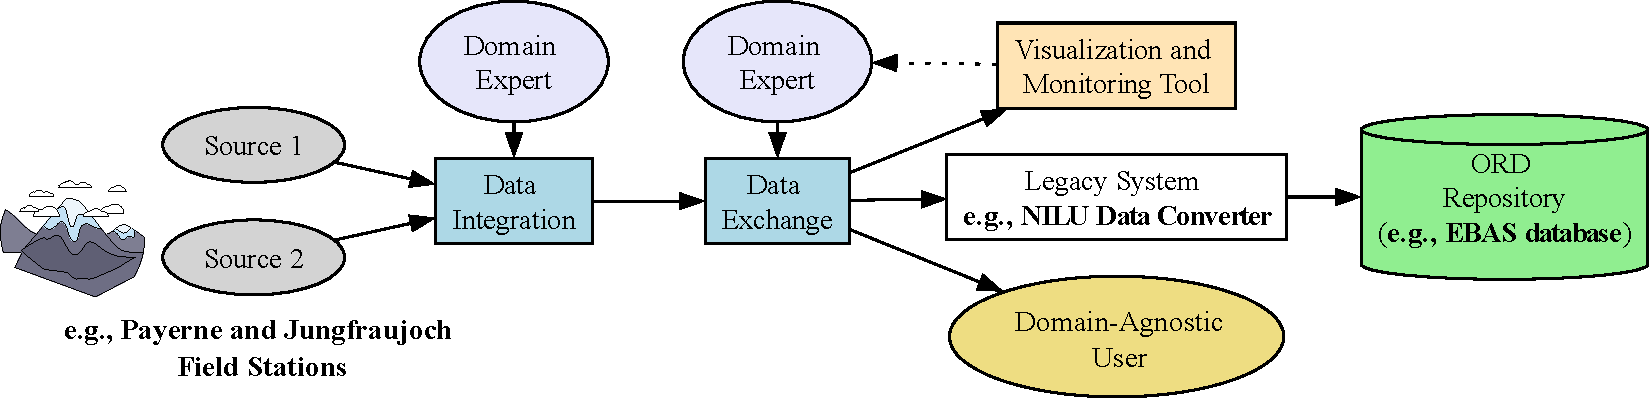
\includegraphics[width=\textwidth]{figures/extended_data_flow_dag_with_actris.pdf}
    \caption{Diagram of the expert-driven FAIR data exchange system.}
\end{figure}


This system, unlike the above implementation, exhibits the following:

\end{block}

\vspace{1em} % Add some space before next block


\begin{exampleblock}{System characteristics:}
\begin{enumerate}
    \item 
    Adaptable to new needs, making it interoperable across users and systems.
    \item 
    Modular, allowing components to be reused, replaced, or maintained independently.
    \item 
    Configurable with domain knowledge supplied externally, supporting expert feedback loops.
    \item 
    Transparent, enabling monitoring of data flows and tracking of data provenance through a clear, structured design.
\end{enumerate}
\end{exampleblock}

\textbf{Practical implementation (Technical stack)}

\begin{figure}[H]
    \centering
    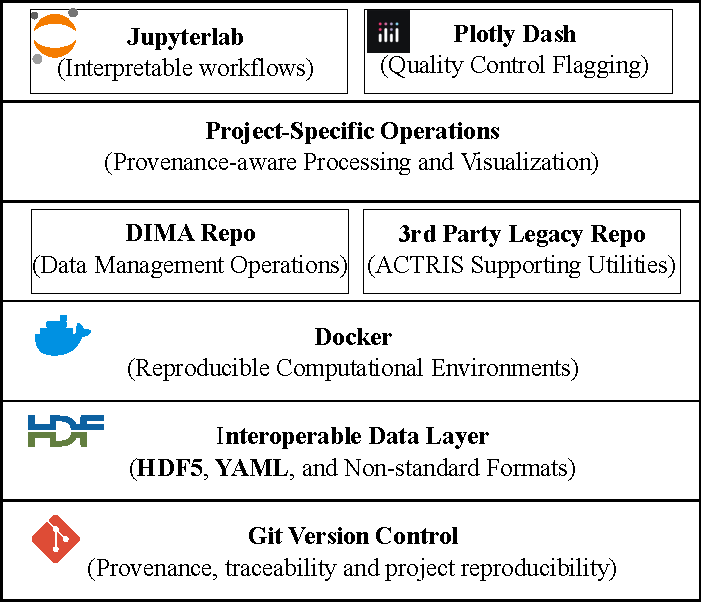
\includegraphics[width=0.5\textwidth]{figures/layered_stack.pdf}
    %\caption{Diagram of the expert-driven FAIR data exchange system.}
\end{figure}

\vspace{0.5em}
\colorbox{lightgray}{
  \parbox{0.95\linewidth}{
    \textbf{Code Repository:} \url{https://gitea.psi.ch/APOG_public/acsmnode.git}
  }
}
\vspace{0.5em}

\end{block}

\end{column}

%\end{columns}

%\begin{columns}[t]

\separatorcolumn

\begin{column}{1.5\colwidth}

\begin{block}{FAIR data chains in ACTRIS Switzerland---Use case}


\textbf{Challenge: }Standardized annual submission of  aerosol composition observations from field stations (\textbf{Payerne} and \textbf{Jungfraujoch}) to the \textbf{EBAS database}.

\textcolor{white}{ }
We consider raw data described in the Table below.
\textcolor{white}{white}
\begin{table}[!ht]
\resizebox{0.75\textwidth}{!}{%
\centering
\begin{tabular}{|c|c|c|}
\hline
\textbf{Data Source} & \textbf{File Formats} & \textbf{Submission Date} \\
\hline
 Aerodyne & TXT, CSV & \multirow{3}{*}{May 31, 2025} \\
Aerosol Chemical Speciation Monitor   & NAS & \\
(ACSM) & YAML & \\
%PTR-TOF MS & NetCDF \\
\hline
\end{tabular}
}
\end{table}

  \end{block}
%\begin{comment}
%\begin{exampleblock}{General data chain properties:}
%\begin{itemize}
%    \item 
%    Standards Compliance: CF convention metadata + EBAS database rules for quality control (flagging)
%    \item 
%    \textbf{Docker} ensures consistent processing across stations and %time periods    
%\end{itemize}   
%\end{exampleblock}
%\end{comment}
%\textcolor{white}{white}
\begin{block}{Configurable Data Integration using YAML files}
     
\textbf{Goal:} Search, Retrieve, and Integrate Raw Data in HDF5 format

\begin{figure}
\centering
%\includegraphics[width=0.65\textwidth]{figures/EarthObservation_HSI.pdf}
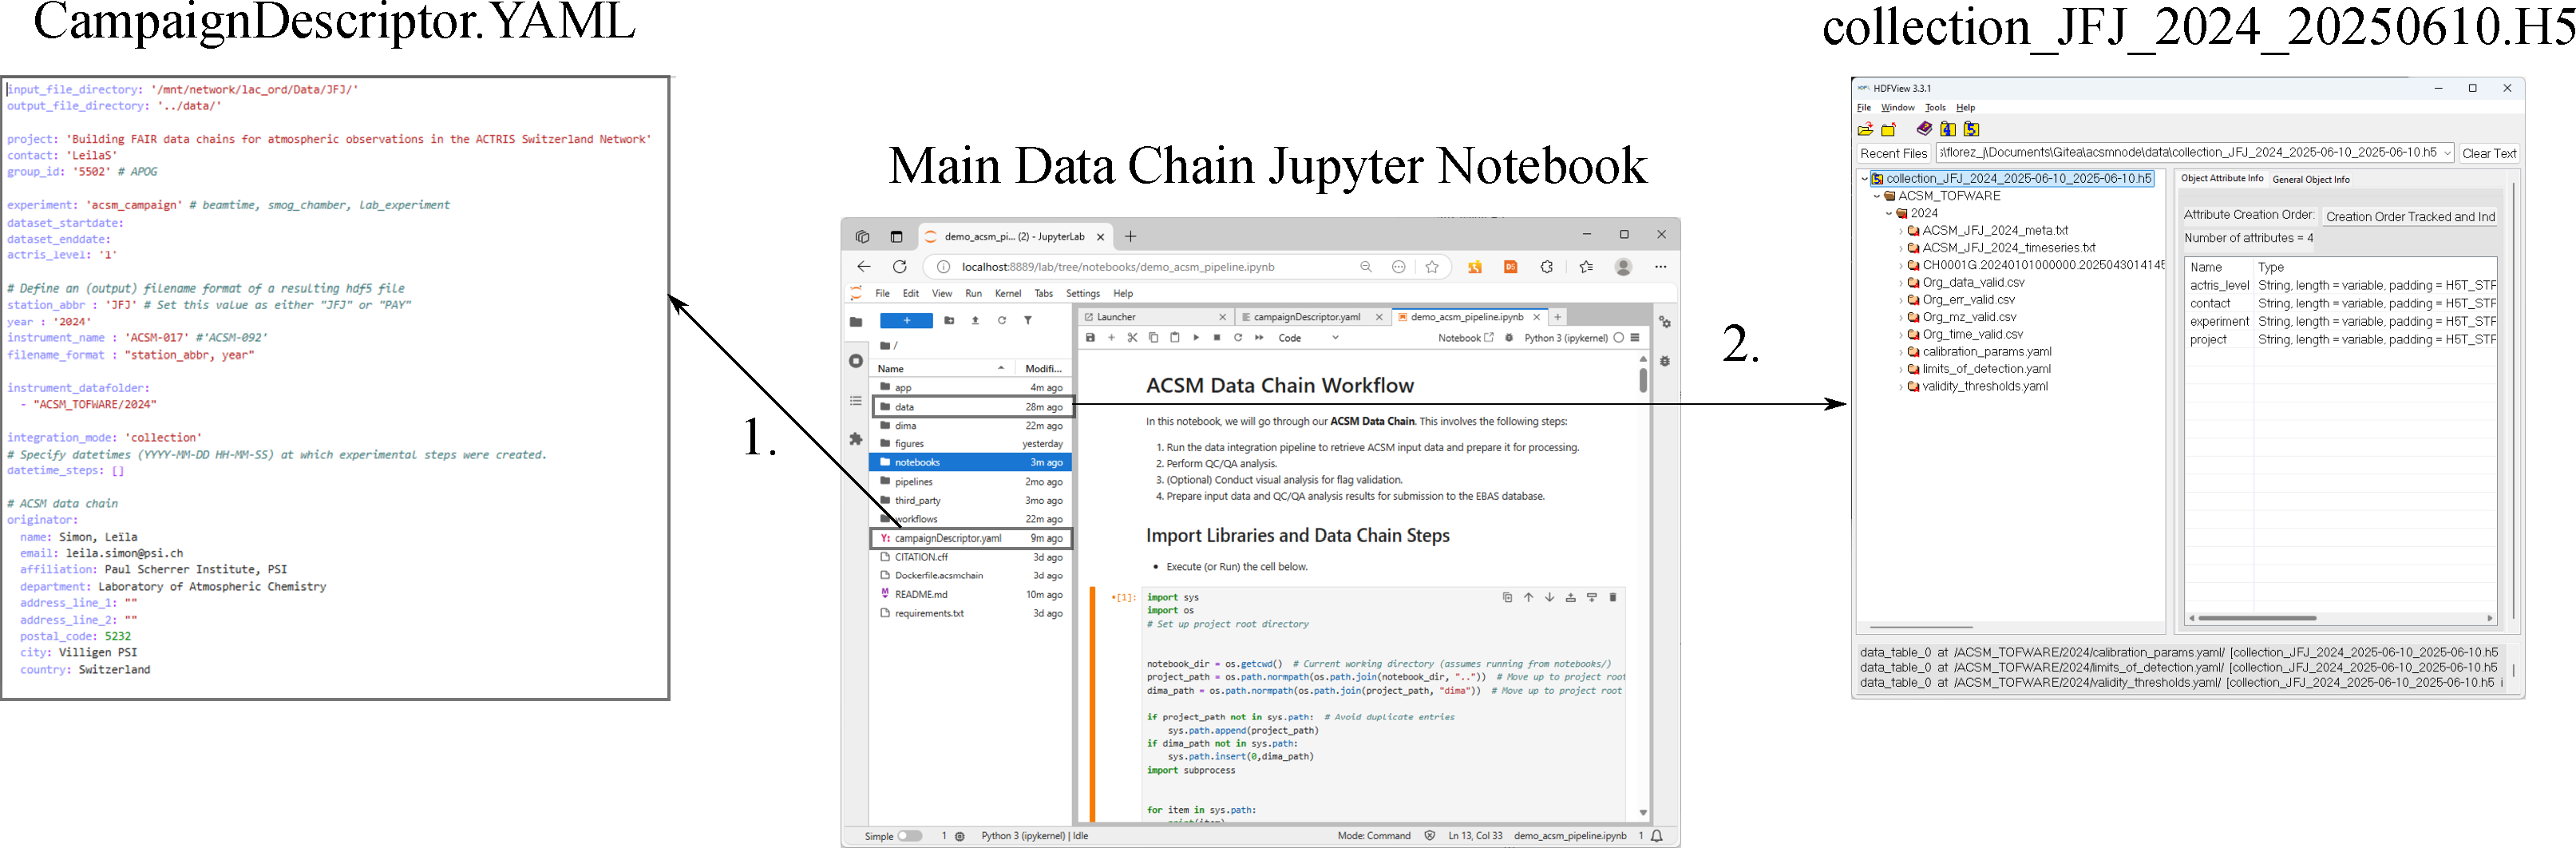
\includegraphics[width=0.7\textwidth]{figures/data_integration_step.pdf}
\end{figure}
\colorbox{lightgray}{
  \parbox{0.95\linewidth}{
    \textbf{Code Repository:} \url{https://gitea.psi.ch/5505-public/dima.git}
  }
}
\end{block} 



\begin{block}{Interactive Data Annotation for Quality Control} % Quality Control Workflow}

\textbf{Goal:} Apply time-dependent correction factors to observations and generate quality control flags with expert validation, complying with EBAS database. 

  \begin{figure}
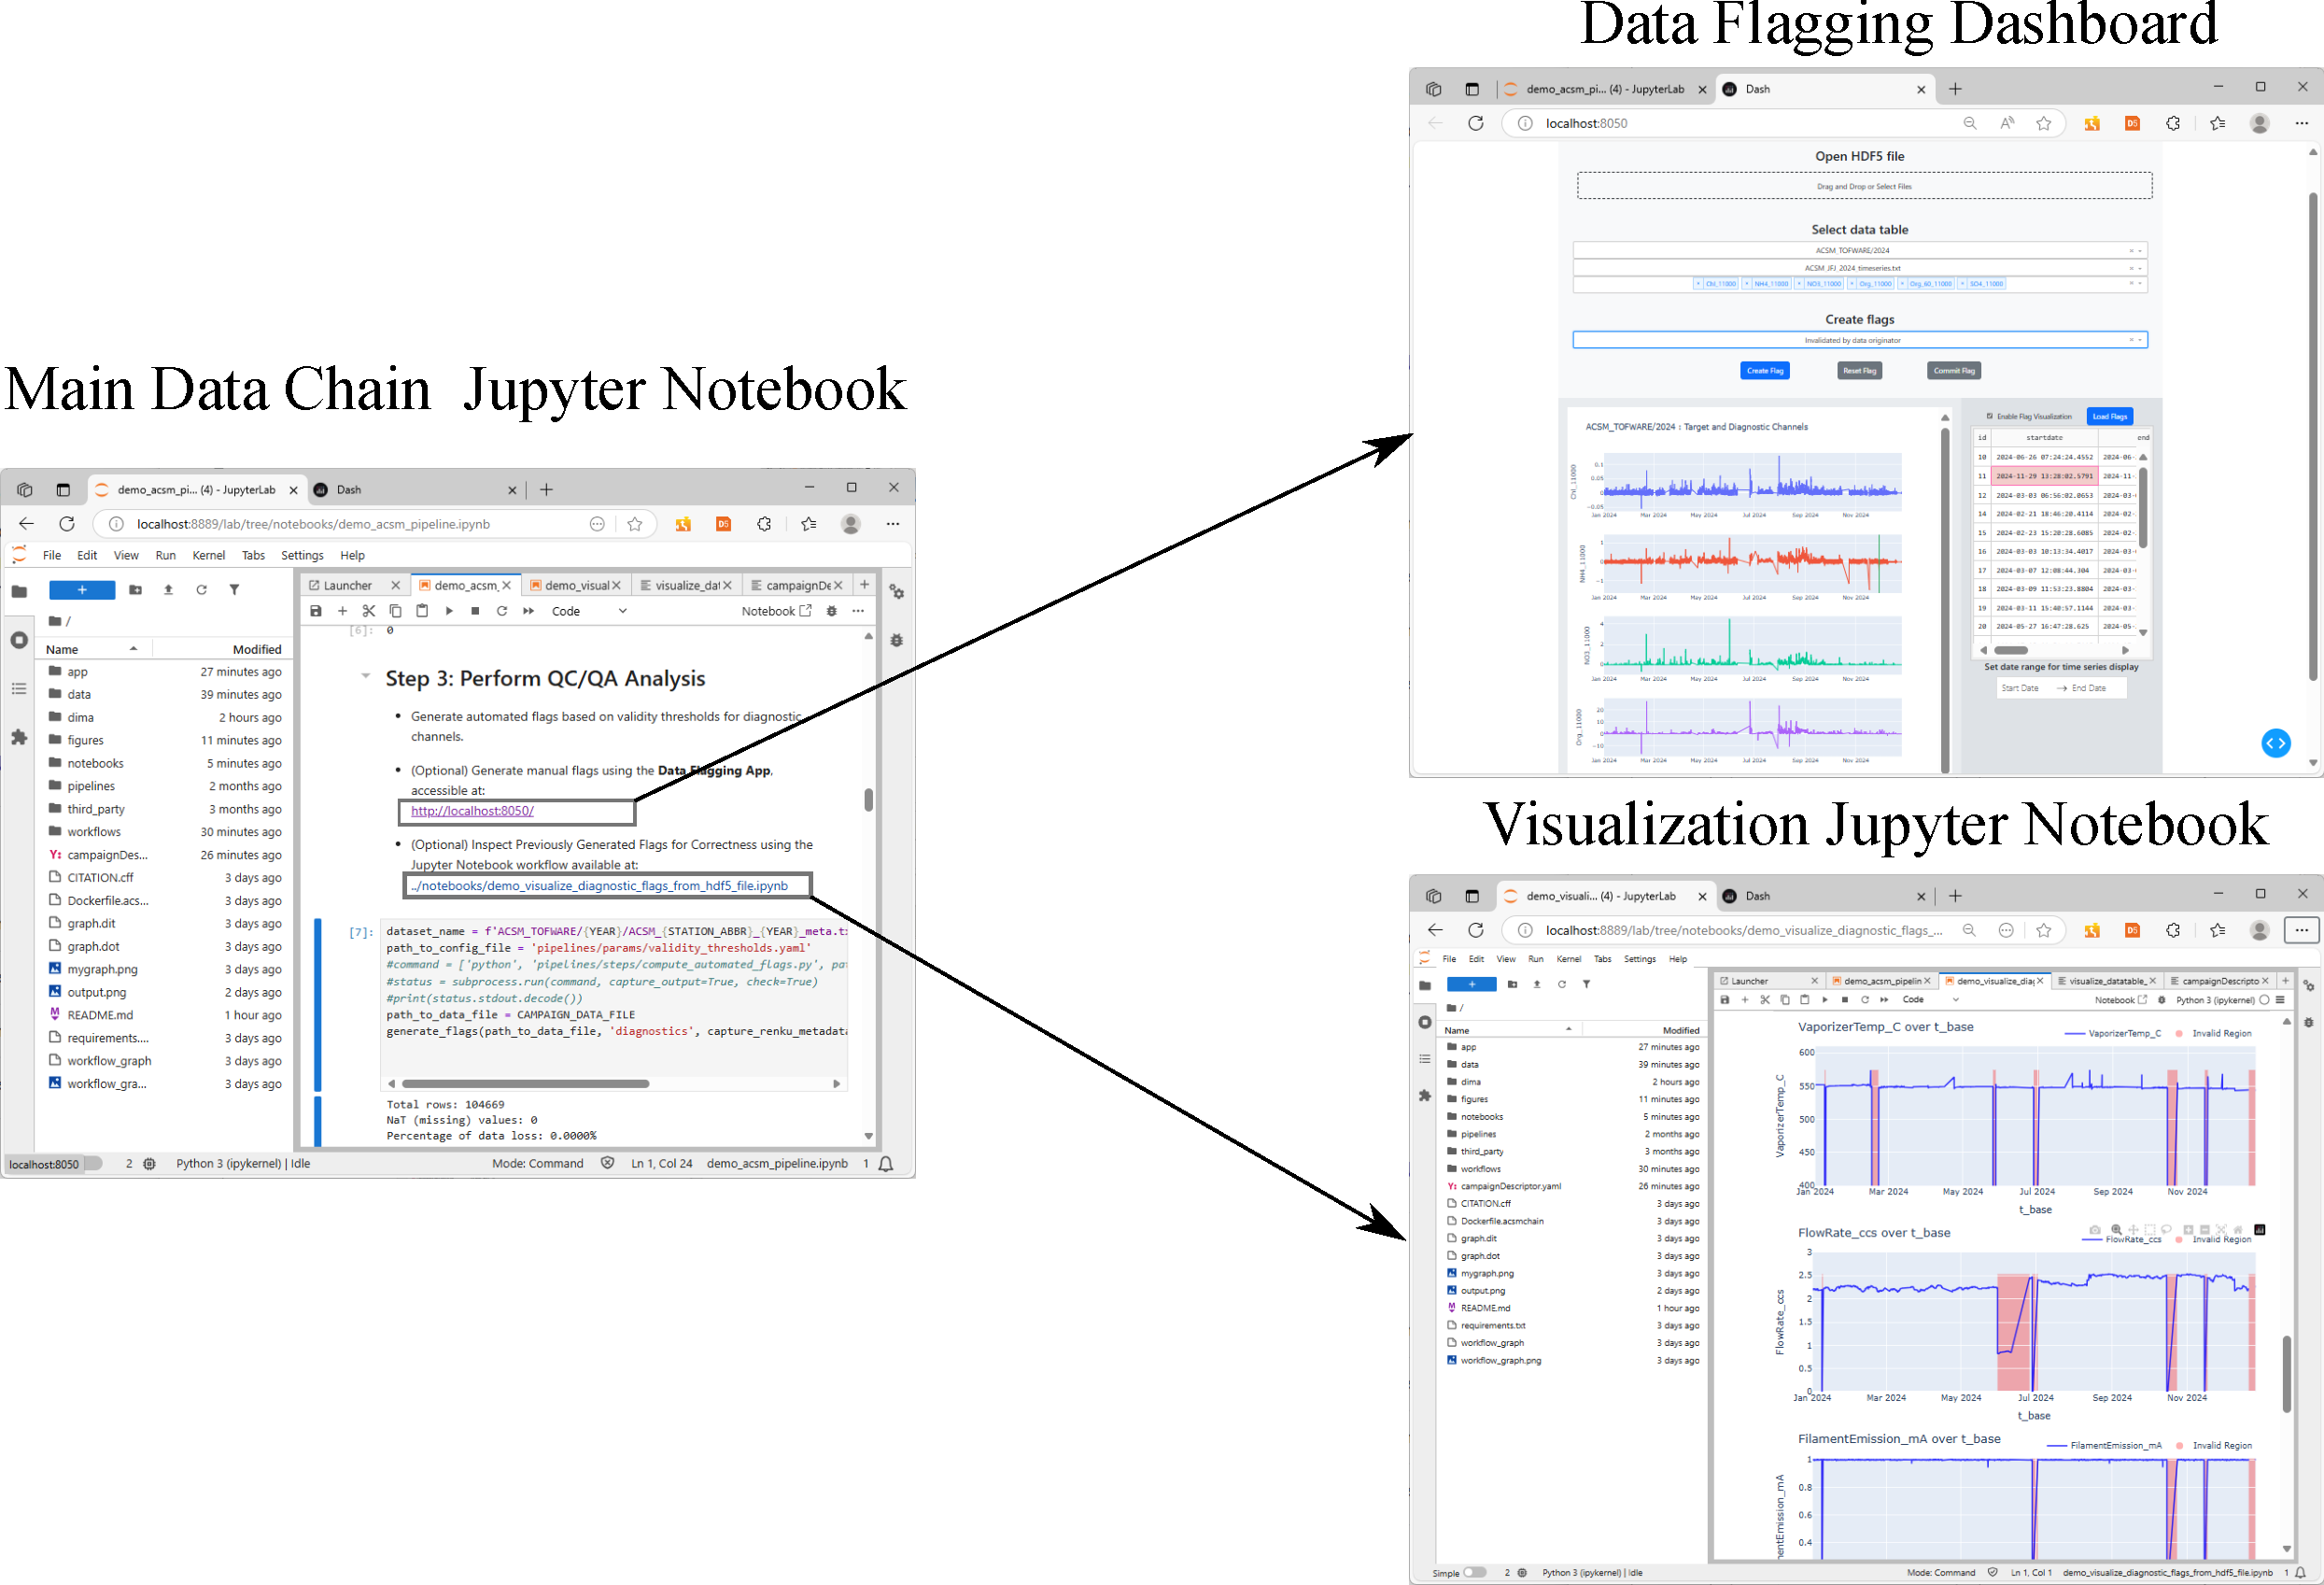
\includegraphics[width=0.6\textwidth]{figures/quality_control_workflow.pdf}
\end{figure}
Enables reconciliation of \textbf{Automatic Diagnostic Flags}, \textbf{Station-specific Flags}, and  \textbf{Manual Review Flags}.
%%\textbf{Features:} Enable reconciliation 
%\begin{itemize}
%    \item \textbf{Automatic Diagnostic Flags}: threshold-based detection of instrument malfunctions.
%    \item 
%    \textbf{Expert Knowledge Flags:} Station operator insights on local conditions and maintenance events and calibration periods.
%    \item 
%    \textbf{Manual Review Flags:} Visual inspection of time series anomalies.
%\end{itemize}

\end{block}

\begin{block}{Accessible Data Products for Domain-Agnostic Reuse}

\textbf{Primary Product:} EBAS-ready files conforming to ACTRIS Level 2 quality standards.

\textbf{Secondary Product:} A comprehensive, self-describing file that integrates:
\begin{itemize}
  \item Original and intermediate data products with rich contextual and provenance metadata, as shown below.

  \begin{figure}
  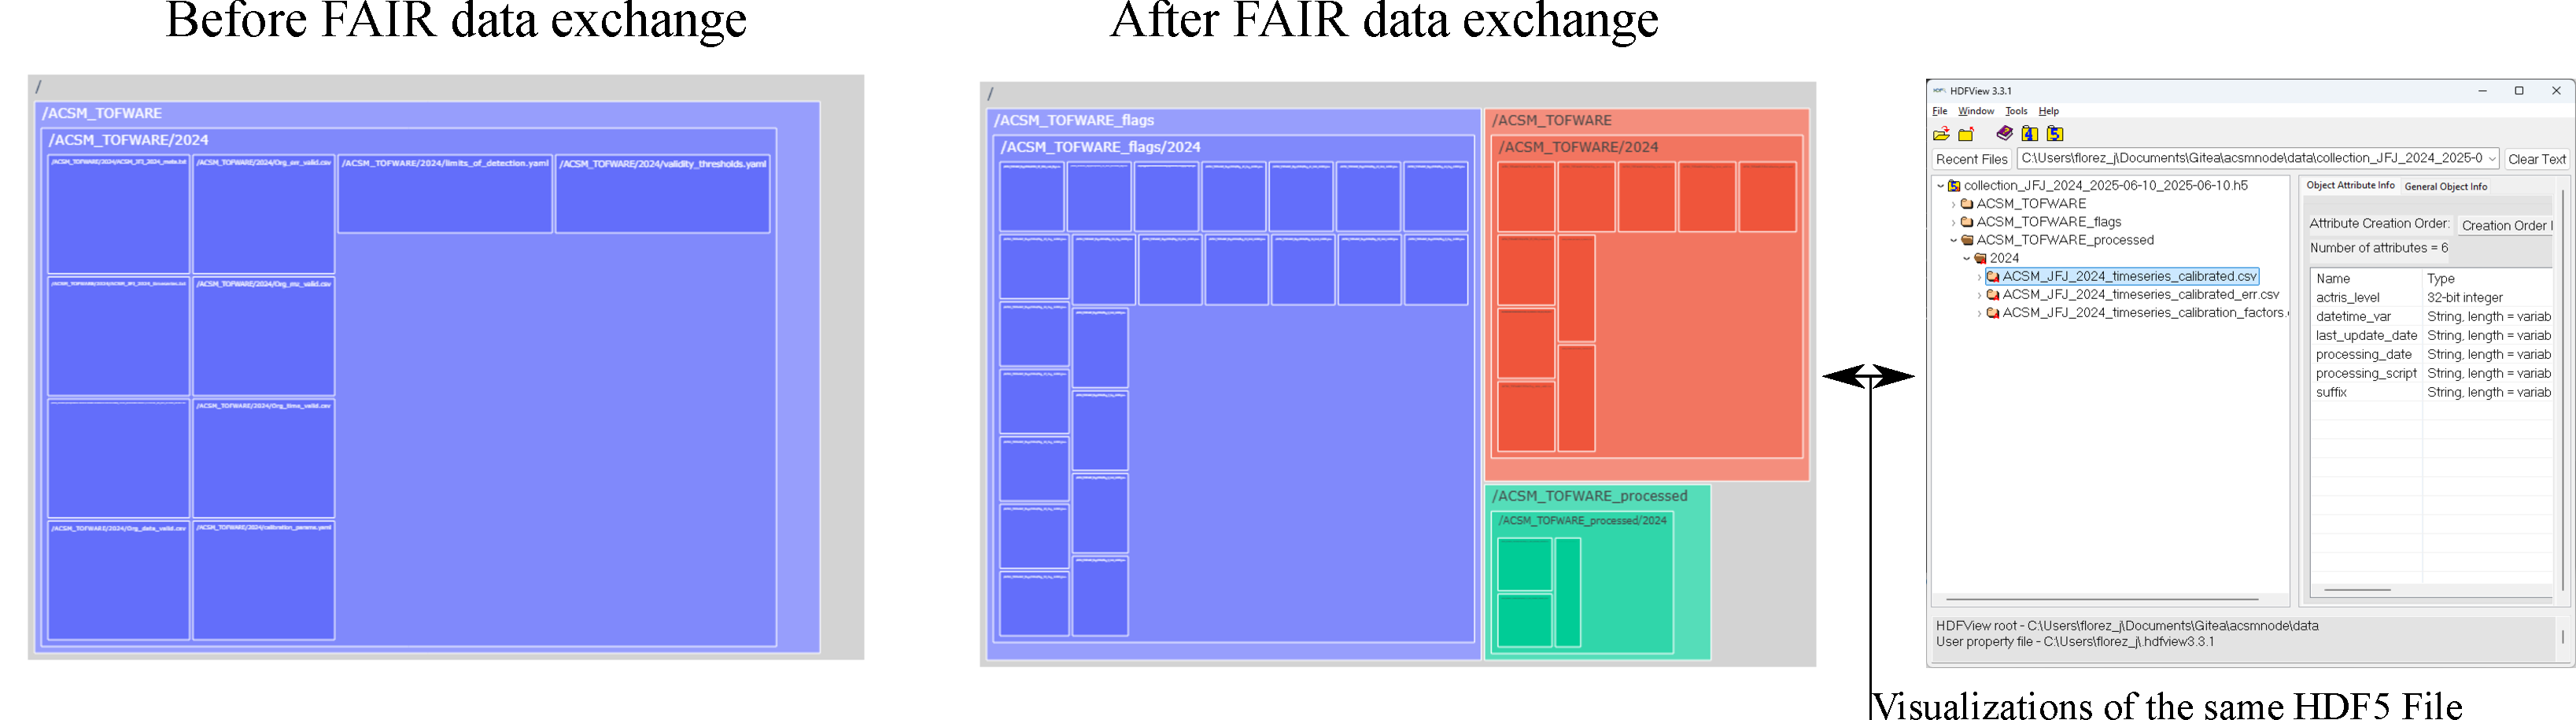
\includegraphics[width=0.9\textwidth]{figures/hdf5_before_after.pdf}
  %\caption{Initial integrated file (left) and enhanced HDF5 file (right)}
\end{figure}
  \item An auto-generated prospective provenance graph in Renku workflow format, visualized as below

\begin{figure}
  \includegraphics[width=\textwidth]{figures/workflow_acsm_data_JFJ_2024.pdf}

\end{figure}
\end{itemize}
\end{block}


  
  %\begin{block}{References}

   % \nocite{*}
   % \footnotesize{\bibliographystyle{ieeetr}\bibliography{poster}}

  %\end{block}

\end{column}

\separatorcolumn
\end{columns}
\end{frame}

\end{document}
